\section{Implementation}

Our system uses input from sensors that inform the controller processor whether bus or other pedestrian are present, and adjust light timing accordingly. Therefore, it's a computerized controller in opposition to electromechanical controller in which the logic stands in hardware (dial timer, motor, relays..).

\subsection{Micro-controller}

We had at our disposition Arduino Uno, Arduino Due, Arduino Yun and Intel Galileo board. We choose the Arduino Due because we feared than we might need more pin I/O pins than other board provide but in the end it was not the case.	But the biggest advantage the Arduino Due provides is that it deliver way more power on the pin.

\subsection{Environment input}

We put button to simulate outside events for bus and pedestrians. We would have used proximity sensor for the bus if we had one available.

\subsubsection{Interruption}

We wired those two button to pins which are attached to an interruption. The rising of current on those pin trigger the interruption (done in hardware).

\subsubsection{ISR}

In our code the Interrupt Service Routine is only setting a volatile boolean to true. We purposely wanted to keep the ISR function as small as possible since it's not possible to interrupt an interruption on an Arduino board.


\subsection{From Uppaal to C}

Thanks to Uppaal, we believe to have a correct theoretical model. We use it to make the C code. Therefore in our code, we have the state and the transition implemented like we can find in Uppaal.

\subsection{Serial monitor}

To be able to detect hardware problems (e.g. desoldered button) and follows the execution of our system, we enabled the Arduino Serial Monitor. Here is an example of a backtrace :

\begin{verbatim}
========= RESET =========
verifier() : OKAY
setup() : initialisation done
crosswalkCall() : ISR : button pressed
crosswalk: Red --> Called
SIGNAL: PEDESTRIAN
trafficLightFrontBack: Red --> Crosswalk
SIGNAL: CHANGE
trafficLightLeftRight: Green --> Red
crosswalk: Called --> Green
SIGNAL: PEDESTRIAN
trafficLightLeftRight: Red --> Crosswalk
verifier() : OKAY
SIGNAL: CHANGE
crosswalk: Green --> Red
SIGNAL: FREE
trafficLightLeftRight: Crosswalk --> Red
trafficLightFrontBack: Crosswalk --> Green
verifier() : OKAY
SIGNAL: CHANGE
trafficLightFrontBack: Green --> Red
trafficLightLeftRight: Red --> Green
verifier() : OKAY
\end{verbatim}

\subsection{Redundant checker}

We defined a function that check if there is a conflicting state in our system (e.g. conflicting green light). It is called at each transition. If it finds something wrong, it proceeds to turnoff all light except an blinking alert LED.


\subsection{Demonstration}

Here is a 2 minutes video that shows what we implemented better than a thousand words description would.

\begin{figure}[H]\label{fig:ytv}
  \centering
    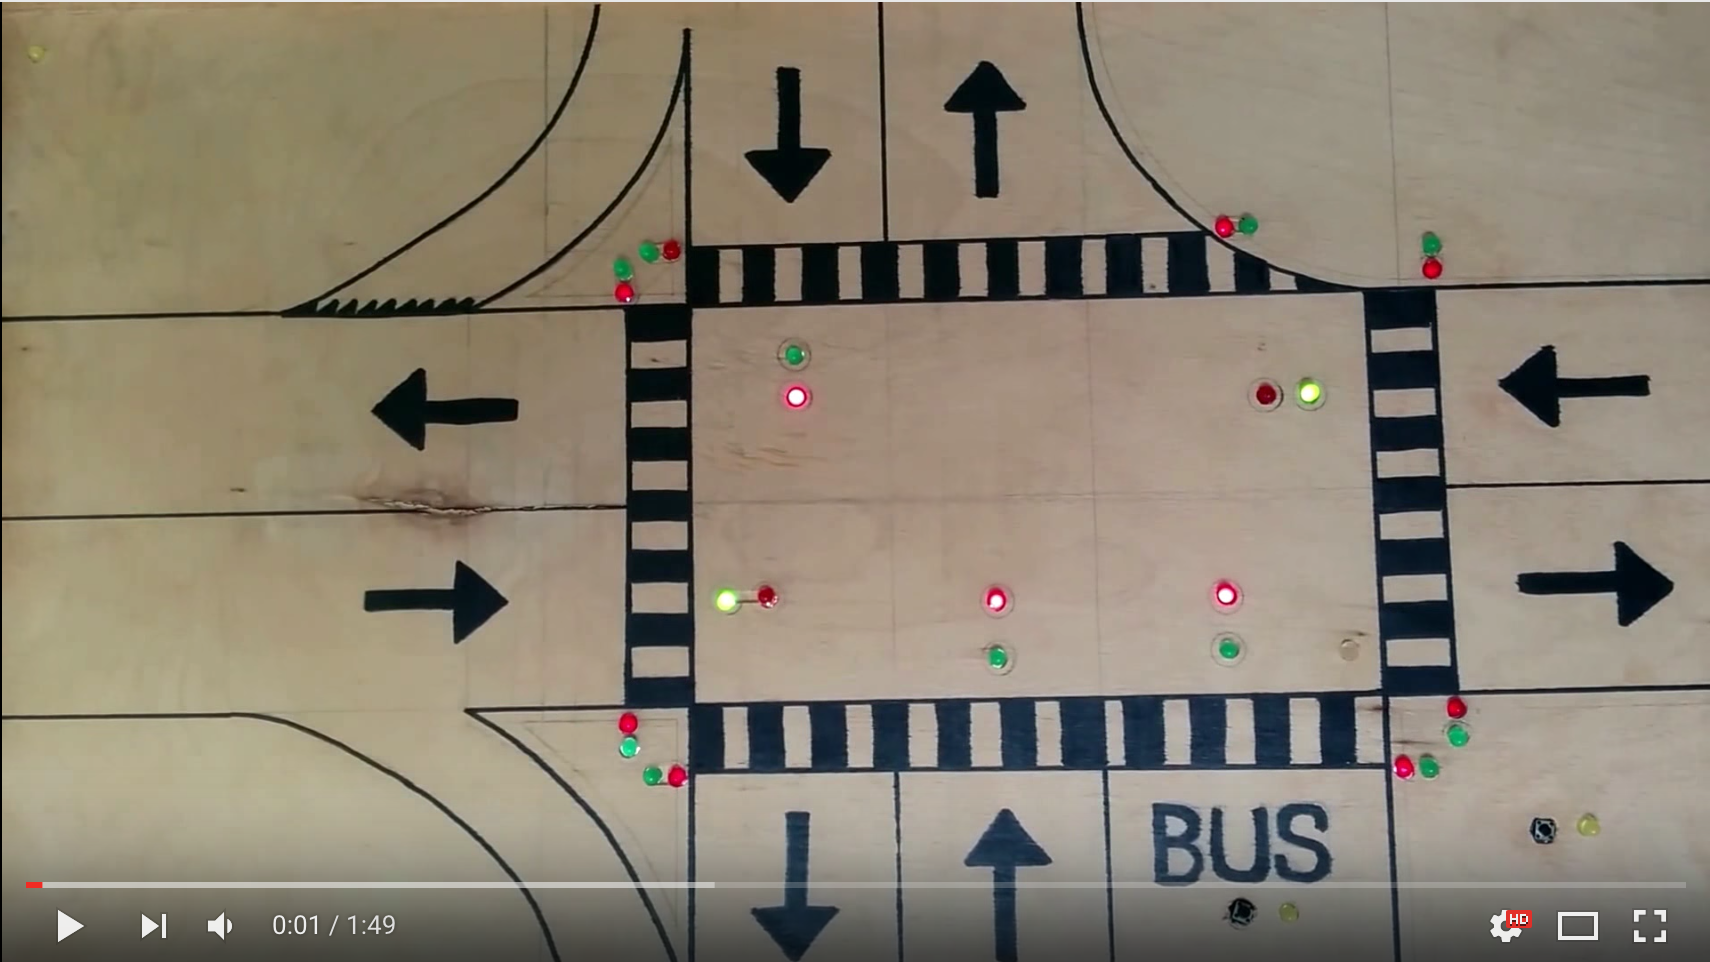
\includegraphics[width=0.7\textwidth]{picture/demo.png}
    \caption{YouTube demonstration}
\end{figure}

It's accessible at :  \url{https://www.youtube.com/watch?v=eleQZ59nWXM}.